\section{Hélice e Aerodinâmica de Propulsores}
\label{sec:helice_aerodinamica}

A hélice é o componente mecânico responsável pela conversão do torque fornecido pelo motor em tração ($T$), constituindo o elemento propulsor essencial em aeronaves de pequeno porte e protótipos de \textit{aerodesign} \cite{McCormick1995}. O princípio de operação baseia-se na rotação de pás com perfis aerodinâmicos que, ao interagirem com o fluido, geram um diferencial de pressão responsável pela força de propulsão \cite{Brandt2015}.


O desempenho de uma hélice é intrinsecamente ligado à sua velocidade de rotação ($n_{prop}$) e à velocidade de escoamento livre ($V_{\infty}$). A caracterização adimensional desse regime de operação é dada pela razão de avanço ($J_{prop}$), definida pela \eqref{eq:razao_avanco}, onde $D_{prop}$ é o diâmetro da hélice \cite{Brandt2015}:

\begin{equation}
    J_{prop} = \frac{V_{\infty}}{n_{prop} D_{prop}}
    \label{eq:razao_avanco}
\end{equation}


Devido à natureza complexa do escoamento helicoidal, a determinação da tração ($T$), do torque ($Q$) e potência, requerida pela hélice é realizada através de coeficientes adimensionais, $C_T$, $C_Q$ e $C_P$, respectivamente. Estes coeficientes são funções da geometria da pá e da razão de avanço, sendo expressos conforme \eqref{eq:ct_model} \cite{McCormick1995, Brandt2015}:

\begin{equation}
    \begin{cases}
        T_{prop} &= C_T(J_{prop}) \cdot \rho n_{prop}^2 \cdot D_{prop}^4  \\
        Q_{prop} &= C_Q(J_{prop}) \cdot \rho n_{prop}^2 \cdot D_{prop}^5 
    \end{cases}
    \label{eq:ct_model}
\end{equation}

\noindent onde $\rho$ é a densidade do ar [kg/m³]. O comportamento típico desses coeficientes é decrescente com o aumento de $J$, visto que o incremento da velocidade de avanço reduz o ângulo de ataque efetivo das pás, diminuindo as forças aerodinâmicas resultantes.

Na literatura clássica de aerodinâmica de baixa velocidade, como nos dados disponibilizados pela \textit{University of Illinois Urbana-Champaign Propeller Database} coordenado pelo Professor Selig, a caracterização experimental de hélices costuma priorizar o coeficiente de potência ($C_P$) em detrimento do coeficiente de torque ($C_Q$) \cite{SeligPropDB}. Essa preferência decorre da aplicação tradicional em motores a combustão, onde a potência disponível é a métrica primária de desempenho.

Entretanto, para a análise de sistemas de propulsão elétrica, o torque requerido pela hélice é a variável de interesse para o acoplamento dinâmico com o motor. A conversão entre essas grandezas é direta e fundamenta-se na relação $P = Q \omega$. Substituindo as definições adimensionais de $C_P$ e $C_Q$, obtém-se a relação expressa por \eqref{eq:cq_from_cp} \cite{SeligPropDB, Brandt2015}:

\begin{equation}
    C_{Q} = \frac{C_P}{2\pi}
    \label{eq:cq_from_cp}
\end{equation}

No mercado de aeromodolismo e competições de \textit{Aerodesign}, as hélices são comumente identificadas por um código alfanumérico que descreve suas dimensões principais, geralmente expressas em polegadas. A nomenclatura padrão segue o formato $D \times P$, onde $D$ representa o diâmetro da hélice e $P$ representa o passo (\textit{pitch}) \cite{Brandt2015}.

O diâmetro ($D$) é a medida de extremidade a extremidade das pás, definindo a área do disco da hélice. Já o passo ($P$) é definido teoricamente como a distância linear que a hélice avançaria em uma revolução completa caso operasse em um meio sólido sem escorregamento \cite{McCormick1995}. Por exemplo, uma hélice $10 \times 7$ possui $10$ polegadas de diâmetro e um passo teórico de $7$ polegadas. 

Adicionalmente, sufixos são frequentemente utilizados para indicar a aplicação ou perfil da pá. O sufixo "E", como em $10 \times 7\text{E}$, designa hélices da categoria \textit{Thin Electric}, que são otimizadas para motores elétricos. Estas possuem perfis mais finos e massas reduzidas, visando maior eficiência em rotações menores se comparadas às hélices destinadas a motores a combustão interna \cite{McCrink2015}.

Para condições da bancada estática é possível considerar que $V_\infty \approx 0 \ [m/s]$, logo $C_T \approx C_{T_{max}}$ e $C_Q \approx C_{Q_{max}}$, fenômeno que é observado na \autoref{fig:Dados_Selig}, onde demonstra os dados experimentais e analíticos lado a lado de duas hélices 10x5 e 10x7.

\begin{figure}[ht]
    \centering
    \caption{Dados Analíticos e Experimentais de Hélice Bipás}
    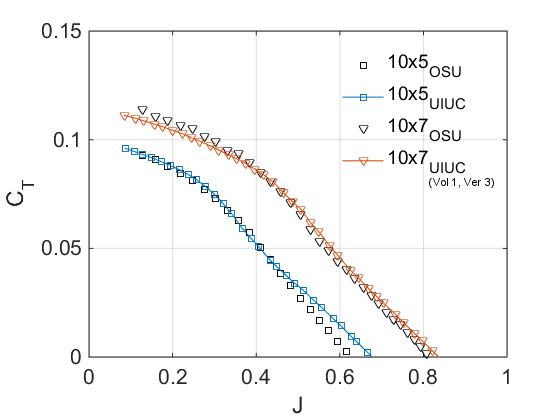
\includegraphics[width=0.4\linewidth]{Textuais/Imgs/Revisao/Selig_propeller_data_ct.png}
    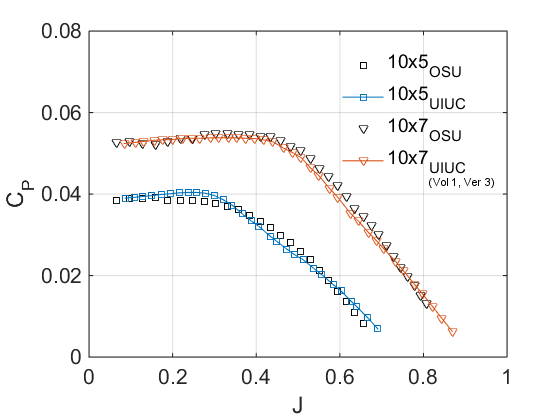
\includegraphics[width=0.4\linewidth]{Textuais/Imgs/Revisao/Selig_propeller_data_cp.png}
    \label{fig:Dados_Selig}

    Fonte : \cite{McCrink2015}
    
\end{figure}

Usando da \autoref{eq:bldc_mecanica} e considerando que a aceleração angular é nula, é possível deduzir $\hat{C_{Q_{max}}}$ e  $\hat{C_{T_{max}}}$ conforme apresentado nas \autoref{eq:Prop_coeff1} e \autoref{eq:Prop_coeff2}.

\[
\hat{T_e} - B \cdot \hat{\omega} - Q_{prop} = 0 
\]
\[
Q_{prop} = \hat{T_e} - B \cdot \hat{\omega} = C_Q (J_{prop}) \cdot \rho \hat{n}^2_{prop} {D}^5_{prop}
\]

E como $V_{\infty} \approx 0 \rightarrow \ J_{prop} = \frac{V_{\infty}}{n_{prop}D_{prop}} \approx 0$ e também $\hat{n}_{prop} = \frac{2\pi}{60} \hat{\omega}$

\begin{equation}
    \hat{C_{Q_{max}}} (\hat{\omega})= \frac{3600 \cdot (\hat{T_e}- B\cdot \hat{\omega}) }{4\pi^2\rho \hat{\omega}^2D_{prop}^5}
    \label{eq:Prop_coeff1}
\end{equation}

\begin{equation}
    \hat{C_{T_{max}}} (\hat{\omega}) = \frac{3600 \cdot T_{prop}}{4\pi^2\rho \hat{\omega}^2D_{prop}^4}
    \label{eq:Prop_coeff2}
\end{equation}

Um fator a se notar das equações é que o $C_{T_{max}}$ e do $C_{Q_{max}}$ são funções da rotação, para um ensaio mais padronizado considera-se que o $\hat{\omega}$ é máximo para o conjunto motopropulsor escolhido, visto que para cada \textit{duty cycle} iremos obter uma rotação diferente e por consequência trações e torque diferentes, por conta da tensões de linha média diferentes, como a importância do ensaio é descobrir esses coeficientes para decolagem onde deseja-se ter uma maior tração ou seja uma rotação máxima.

\subsection{Característica de Carga e Acoplamento Dinâmico com o Motor}
\label{sec:helice_acoplamento}


A determinação com precisão do desempenho máximo do conjunto motopropulsor não pode ser baseada apenas nas características isoladas de cada componente. O comportamento real do sistema é definido pelo acoplamento dinâmico entre o torque disponível do motor e o torque requerido pela carga. O ponto estável de operação do sistema completo é a intersecção dessas duas curvas, conforme ilustrado na \autoref{fig:tik_acoplamento_bldc_helice}.

\begin{figure}[ht]
    \centering
    \caption{Ponto de Operação Dinâmico}
    \begin{tikzpicture}
        \begin{axis}[
            axis lines = left,
            xlabel = {Rotação Mecânica ($\omega$) [pu]},
            ylabel = {Torque ($T$) [pu]},
            xmin=0, xmax=1.5,
            ymin=0, ymax=1.2,
            xtick={0, 0.5, 1.0, 1.5},
            ytick={0, 0.5, 1.0, 1.5},
            grid=both,
            grid style={dotted, gray},
            legend style={at={(0.95,0.95)}, anchor=north east, nodes={scale=0.8}},
            height=7cm,
            width=12cm,
            legend style={
                at={(0.97,0.03)}, 
                anchor=south east, 
                nodes={scale=0.8, text=black}, % Texto sempre preto
                cells={anchor=west}
            },
        ]
        
        % Curva do Motor em PU
        % Zona 1: Torque constante até a rotação base (w = 1)
        \addplot[domain=0:1.0, blue, thick, name path=motor2, forget plot] {1};
        % Zona 2: Enfraquecimento de campo (T decai com 1/w)
        \addplot[domain=1.0:1.5, blue, thick, name path=motor] {1/x}; 
        \addlegendentry{Torque Motor}
        % Curva da Hélice em PU
        % Modelo proporcional a w^2. O coeficiente (ex: 0.6) define o "peso" da hélice.
        \addplot[domain=0:1.5, red, thick, name path=helice] {2*x^2};
        \addlegendentry{Torque Hélice}
        % Encontra a intersecção automaticamente
        \path [name intersections={of=motor2 and helice, by={point1}}];
        
        % Marca o ponto de intersecção
        \fill (point1) circle (2.5pt) node[above left=0.1cm, fill=white, inner sep=1pt, draw, rounded corners, scale=0.8] {Ponto de Operação};

        % Linhas tracejadas de auxílio para os eixos (usando projeção ortogonal |- e -| para evitar erros de compilação)
        \draw[dotted, thick] (point1) -- (point1 |- {axis cs:0,0}) node[below, fill=white, inner sep=2pt] {\scriptsize $\omega_{op}$};
        \draw[dotted, thick] (point1) -- (point1 -| {axis cs:0,0}) node[left, fill=white, inner sep=2pt] {\scriptsize $T_{op}$};

        \end{axis}
    \end{tikzpicture}
    
    \label{fig:tik_acoplamento_bldc_helice}
    \vspace{0.2cm}
    \small Fonte: Autor (2026).
\end{figure}

O ponto de intersecção na \autoref{fig:tik_acoplamento_bldc_helice} representa o único ponto de operação estacionário possível para aquele par específico de motor e hélice.
